\Chapter{My Father}{Glyn Court}

\quotemark{If it were permitted to contradict a lady}, as said the gallant Mr Elton, I would take issue with my wife’s statement that one would be hard put to it to name a date or place having a supreme significance in our particular portion of history. I would identify it as a moment in April 1876, when a baby was born in the village of Roadwater. That baby, after a considerable delay, as is only natural, became my father, and obviously, but for him we should have no story to tell. And as young William George, or \quotemark{Will} to the family, figures so largely in the following pages, this seems the right time - and I write this on 6th April 1976, the hundredth anniversary of his birth - for me to essay a portrait of him, not only as he is limned in the memory of a son but also as others recollect him. To know the kind of man he was will help to explain the vagaries of the experiences recounted hereafter; but more, he was a countryman of a type now rarely met with, and some such account will help to preserve the savour of a vanished age.

His father, also William, was the village shoemaker or cordwainer, enjoying, in the mid 1870’s, a brief spell of modest prosperity. Will, in the heady days of the first Education Act, was sent to the village school on the breezy hillside of Leighland a mile away, and worked his way contentedly up through the standards to the age of eleven, learning the three R’s, spelling history and geography and acquiring a beautiful hand. He would say wistfully, \quotemark{I wish I’d been born with a good memory,} but nobody else noticed any deficiency. Still, authority, in its paedagogic Victorian form, fell out with him when he was eleven. \quotemark{William Court}, thundered bearded Authority, \quotemark{come out to the front}. William came out, feeling he had done nothing to deserve a beating and determined not to have one. As the headmaster raised his cane, William also raised his hand, grasped the goatee beard and clung on for dear life; swish and slash as he might, not a single cut landed and William could claim the victory. But not outstaying his welcome he sped through the door and off home. His father, to his amazement, was highly diverted, but that was William's last day at school, and in later years, feeling the loss keenly, he made painstaking and largely successful efforts to acquire the knowledge of which he had been summarily deprived.

It was in his chosen art of carpentry, for which he served his apprenticeship, that he first found the way to excel, being entrusted with the finishing work at sixpence-farthing an hour, a farthing above the normal wage and a substantial advantage with a sixty-hour week. But by a pleasing quirk of nature, even in his best work his consciousness and craftsmanship were enlivened by flashes of the wayward West Countryman - though I will not say plain, downright dilatory. The parish church of Luxborough, in the late 1890s, was undergoing \quotemark{restoration}, and the firm of carpenters in Dunster for whom he worked were asked to provide an oaken pulpit for some weeks later, when with ecclesiastical junketings the church would be re-opened. Will, as the craftsman, had the commission and set to work. The day of the re-opening drew near, but the pulpit did not; the morning came, the pulpit did not; the bishop came, but still no pulpit; and long was the luncheon enjoyed by his grace while a cart trundled over from Dunster and a perspiring team manhandled the pulpit into place. It would be uncharitable to assume that my father meant to keep the bishop cooling his heels, but one may have one’s thoughts.

\begin{figure}
	\centering
     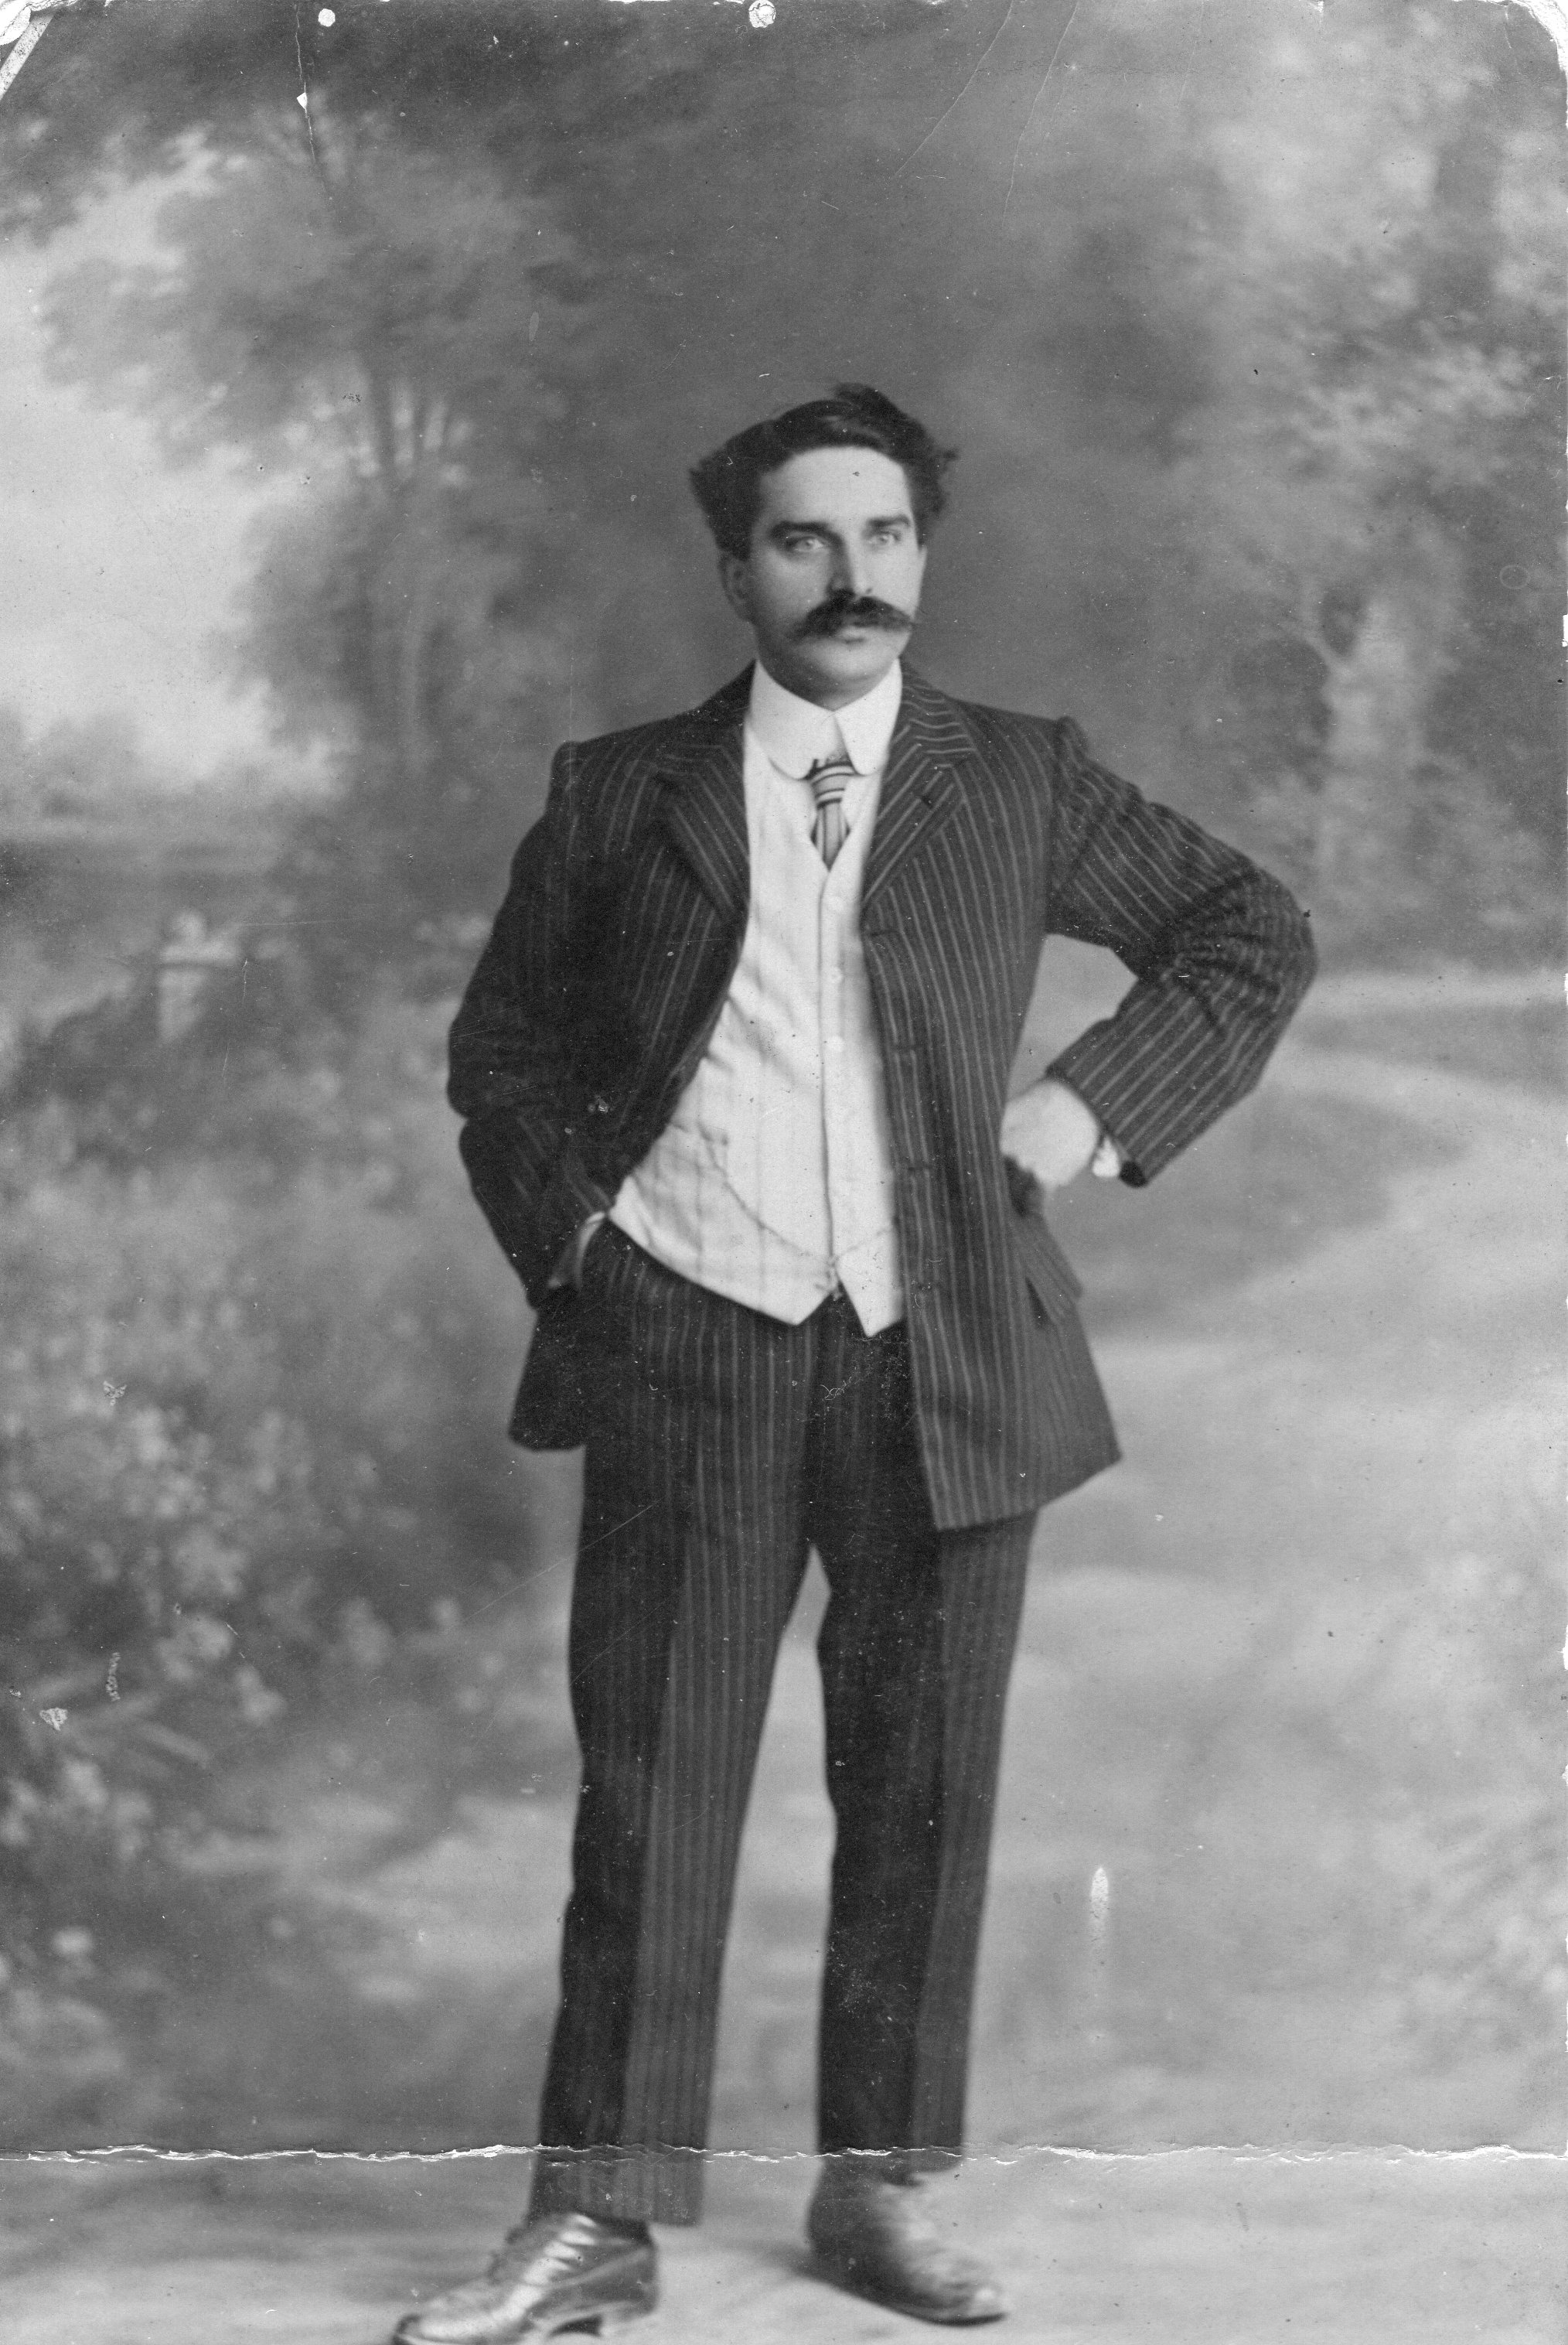
\includegraphics[width=1\textwidth]{figures/WilliamCourt}
     \caption{William Court}
     \label{fig:WilliamCourt}
\end{figure}

In his middle twenties his health failed and he gave up full-time carpentry and became the postmaster of his native village, combining this with a retail extension of his father’s boot end shoe trade. At the same time he fell in love with my mother and should rightly have been able to offer marriage; but my father was not one to hurry things and mother was content to wait; and then came one thing and another - the Great War for one - and Will, such is the power of Family, felt he had to provide for the children of a married sister deserted by her husband; and then a favourite sister cared for him devotedly until she died; and by the time he ventured, into marriage, forty-four years had stolen upon him and, he said, ”I’ll never get married so young again”. But of the ideal happiness of that marriage I will not now speak.

He had, it almost goes without saying, a strong religious faith, for he was born into that sturdy, democratic tradition of Bible Christian Methodism which originated in North Devon and flourished so astonishingly throughout the West of England and the Channel Isles and even in Canada, Australia and Yunnan. All his childhood memories were linked to the crowded congregations and the plain, foursquare chapels whose beauty, invisible to the casual beholder, is seen in the light of the memories and associations which gather round them. Moreover, the social life of the members centred on the chapels, with their choirs and orchestras, and my father, who had a good, true tenor voice and loved music, found in them the companionship of artistic experience. In his early twenties he offered for the Bible Christian ministry in the footsteps of his brother, but family circumstances held him back, and he settled for the ministry of a local preacher and exercised it for half a century.

% Add Picture of William Court

With his Methodist faith, inevitably, came his Liberal one, and although the most peaceable soul alive he revelled in political argument, even though he would have acknowledge Goethe’s aphorism that \quotemark{against stupidity the gods themselves fight in vain}. He worked hard and long for the cause, canvassing, speaking, chairing meetings, and even in the long years of Liberal Eclipse his commitment did not waver. He did not live to see a Liberal revival, but he found a measure of compensation in working for the election of one of the most distinguished Independent Members of Parliament, Vernon Bartlett. But preaching and politics could not fill up the measure of his time, and as his trade achieved a little prosperity - for he was sociability itself, and our progress along the street of a strange town was in the nature of a conversational pilgrimage, with frequent halts to exchange courtesies and comments with complete strangers - he turned to local government and served as chairman and member of the rural district council, as school governor and as Chairman of the parish council for more than a decade. It was in this work that he found his forte, for he was a man to whom most of the village would come for help or advice - with just enough exceptions, such as the following, to remove any likelihood of conceit:

\begin{quote}
\textbf{Clerk to the Parish Council}: The vote for the office of Chairman is as follows: W.G. Court: For, 53; Against, 0.

\textbf{Mr Tiler} (a determined antagonist): Thik’s wrong, Mr Clurk, there’s on’y fifty-three o’ us yere, an’ I didn' vote for ’en!
\end{quote}

My father usually had too low an opinion of himself-largely, I think, because he had not acquired the academic and theological learning of his elder brother - but this story he used to tell with relish, and I am glad of it, because he was then responding to other people's consciousness of his worth. Like most of us, he had a few chronic defects, in his case unpunctuality which could sometimes amount to inconsiderateness, and a few foibles: in thirty years of driving he never apprehended that other motorists had discovered our narrow lanes and might indeed wish for a share in them. But as I look back at my father through the mists of twenty years, I know that these flaws count for little or nothing, and I see, above and beyond all else, one who was kind, gentle and good, by conviction a Christian, by nature a gentleman, are one who lived each day for the unending tomorrow.